\documentclass[a4paper]{jpconf}
\usepackage{graphicx}

\usepackage{amsmath}        % extensions for typesetting of math
\usepackage{amsfonts}       % math fonts
\usepackage{amsthm}         % theorems, definitions, etc.
\usepackage{amssymb}

\usepackage{fancyvrb}       % improved verbatim environment
%\usepackage{natbib}         % citation style AUTHOR (YEAR), or AUTHOR [NUMBER]
%\usepackage[nottoc]{tocbibind} % makes sure that bibliography and the lists
 \usepackage{subfig}

\bibliographystyle{iopart-num}
%\usepackage{citesort}
%% \usepackage[square,sort&compress]{natbib}
\usepackage{iopams}
%\newcommand{\BibTeX}{Bib\TeX}
\newcommand{\REVTeX}{REV\TeX}
\usepackage{bm}
\usepackage{cleveref}

\graphicspath{ {./img/} }

\begin{document}

\title{Geometric Properties of Ising model on an Interacting Self-Avoiding Walks}

\author{Ilya Pchelintsev, Kamilla Faizullina, Evgeni Burovski}
%
\address{HSE University, 101000 Moscow, Russia}


% абстракт и введение я напишу немного позже, когда будет более полное
% осмысление работы

\begin{abstract}
    This is an abstract and that's really abstract.
\end{abstract}

\section{Introduction}

The model of self-avoiding walks is one of extensively studied examples of linear polymers. Moreover, it is the simplest model to study critical behaviour while other models polymer chains have different states in the thermal equilibrium in various solvent conditions. By adding interaction between nearest neighbors of monomers of the walk, we are allowed to study phase transition fixed between solvent conditions, so the given polymer in the thermal equilibrium become extended in good-solvent conditions and collapsed in poor-solvent one. This tricritical nature was described in Ref.\cite{Gennes1979}.

The impact of close-range interaction was studied precisely in models of magnetic polymers, where interaction between monomers became more complex after each monomer carried a spin and strength of nearest neighbors coupling became variable. This is so called Ising Model on a SAW conformation. In Ref.\cite{Garel1999}, the model was complicated by adding external magnetic field and all conclusions about magnetic properties were by comparing with mean-field model. However, there are some geometric properties which impact of magnetic properties is not clear while studying of require more brute methods. 

In previous studies, it was established that Ising model on the self-avoiding walk conformations (SAWs) has a continious type of phase transition \cite{faizullina2021critical}. In this work, we continue study geometric properties of this model and compare them with "papent" models and its modifications, such as Ising model on the rectangular lattice, considered in Ref.\cite{Selke2006}, and two-dimensional interacting self-avoiding walks exactly in their respective critical regions. We suggest that models with similar geometric properties will also have same magnetic propertries, what we suggest to observe in comparing values of Binder cumulants in the $\theta$-transition of models with the equal values of asphericities.

\section{Models and Methods}
In the paper we consider several models: the first one is Ising model on interacting self-avoiding walk from Ref. \cite{faizullina2021critical}, on three different lattices: 2D-square lattice, 3D-square lattice and 2D-triangular lattice. The main difference between square and triangular lattice in defining two additional diagonal monomers on lattice as nearest too. Considering the case of lack of outer magnetic field in this work, the Hamiltonian of the model of fixed conformation $u$ with length $N$ and strength of nearest-neighbors interaction $J$ reads:

\begin{equation}\label{eq:H_Ising_ISAW}
  H_{u, N, \{\sigma\}} = - \sum_{\langle i,j \rangle} J  \sigma_{i}  \sigma_{j},\ \ i,j \in u,\ |u| = N
\end{equation}

The summation runs through spins involved in conformation and only with the nearest neighbors. 

The equlibrium partition function corresponding to Eq.\ \eqref{eq:H_Ising_ISAW} reads
%
\begin{equation}
Z =\sum_{u \in \mathcal{U}_N} \sum_{\{\sigma\}} e ^{-\beta H_{u, N, \{\sigma\}} },
\label{eq:Z}
\end{equation}
%
where $\beta$ is the inverse temperature.

The second model considered in this paper is the Ising model on the rectangular lattice from the Ref.\cite{Selke2006}. Simulated lattices has $L \times rL$ spins and the Hamiltonian is calculated through interaction between all spins and their nearest neighbors respectively:

\begin{equation}\label{H_Ising_Rectan}
  H_{L, r, \{\sigma\}} = - \sum_{\langle i,j \rangle} J  \sigma_{i}  \sigma_{j}
\end{equation}

Here the $i$-th spin of the lattice has a pair of coordinates from $[1..L] \times [1..rL]$. For comparing magnetic properties of models with similar geometric ones we also define shape factors, such as gyration tensor of system with $N$ points $w_{i}$ \cite{Caracciolo2011}:

\begin{equation}\label{eq:Ten_G1}
    Q_{N,\alpha\beta} = \frac{1}{N} \sum^{N}_{i=1}(w_{i,\alpha} - w_{c, \alpha})(w_{i,\beta} - w_{c, \beta})
\end{equation}

where $N$ is length of the system (number of monomers in conformations of Ising-ISAW models or number of spins in the lattice in rectangular Ising), and  $w_{i, \alpha},w_{i, \beta}$ are the coordinates of $i$-th point of conformation. $w_{c, \alpha},w_{c, \beta}$ are coordinates of the center of system (so, $Q_{N, xx}$ and $Q_{N,yy}$ can be defined as mean squares of coordinates of the points of the model in the cartesian coordinate system with the center in the center of model). Eugen values $q1$, $q2$ of given tensor can be interpreted as $Q_{N, xx}$ and $Q_{N,yy}$ in the coordinate system of eugen vectors, or more important - as square of semi-axes of ellipse of inertia of given system. The proportion of them for systems with length $N$ will be \cite{Caracciolo2011}: 

\begin{equation}
    r = \sqrt{\frac{\langle q_{1}\rangle_{N}}{\langle q_{2} \rangle_{N}}}
\end{equation}

Eugen values $q1$, $q2$ are also used in enumerating another important shape factor - mean asphericity \cite{Caracciolo2011}:

\begin{equation}
\label{eq:Asphericity}
    \mathcal{A} = \left\langle \frac{(q_{1} - q_{2})^{2}}{(q_{1} + q_{2})^{2}} \right\rangle_{N}
\end{equation}

The compared magnetic property of our models is the fourth order cumulant of the magnetization of the Binder cumulant, defined as \cite{Binder1981_Ising}:

\begin{equation}
\label{eq:Cumulant}
U_{4} = 1 - \frac{\langle m^{4} \rangle}{3 \langle m^{2} \rangle^{2}}
\end{equation}

Where $\langle m^{4} \rangle$ and $\langle m^{2} \rangle$ are mean fourth and second order of mean magnetization per spin respectively.

We also need to define mean proportion of monomers with fixed number $i$ of nearest neighbors $\langle n_{i} \rangle$, which is counted directly for every monomer in every simulated conformation of walk.

We are interested in comparing models in their respective critical regions. For each structure, critical temperatures of Ising models are known as:

\begin{table}[h]
    \centering
    \begin{tabular}{|c|c|c|}
        \hline
        Structure & lattice & $J_{c}$ \\ \hline
        ISAW conformation & Square & $0.8340(5)$\cite{faizullina2021critical} \\ \hline
        ISAW conformation & Cubic & $0.5263 \pm 0.055$\cite{Foster2021}\\ \hline
        Regular lattice & Rectangular & $\ln{(1 + \sqrt{2}) / 2}$\cite{Onsager}\\ \hline
    \end{tabular}
    \caption{Known values of critical temperature of different modifications of Ising-ISAW model and normal Ising on the rectangular lattice}
    \label{tab:Ising_T_c}
\end{table}

\begin{table}[h]
    \centering
    \begin{tabular}{|c|c|}
        \hline
        lattice & $T_{c}$ \\ \hline
        Square & $0.6673(5)$ \cite{Caracciolo2011} \\ \hline
        Cubic & $0.2779 \pm 0.0041$\cite{Tesi1996} \\ \hline
        Triangular & $ 0.405 \pm 0.07$\cite{Privman1986} \\ \hline
    \end{tabular}
    \caption{Known values of critical temperature of different modifications of ISAW model}
    \label{tab:ISAW_T_c}
\end{table}

% сюда немного позже добавлю критические значения для модели SAW

% Стоит ли добавлять рисунок шага алгоритма 
% и более подробное объяснение методов?? Поскольку ничего не было добавлено, % я решил не расписывать, но описание методов получилось крайне немногословным))


%%%%%%%%%%%%%%%%%%%%%%%%%%%%%%%%%%%%%%%%%%%%%%%%%%%%%%%%%%%%%%%%%%%%%%%%%%%%%%%%
\section{Results}
%%%%%%%%%%%%%%%%%%%%%%%%%%%%%%%%%%%%%%%%%%%%%%%%%%%%%%%%%%%%%%%%%%%%%%%%%%%%%%%%


%%%%%%%%%%%%%%%%%%%%%%%%%%%%%%%%%%%%%%%%%%%%%%%%%%%%%%%%%%%%%%%%%%%%%%%%%%%%%%%%
\subsection{Mean Asphericity and Critical Cumulant}

% если я правильно понимаю, данную подсекцию можно полностью взять из отчёта
% (9.6), как раз данная часть больше всего похожа по содержанию на Results -
% план действий (какие длины были взяты, под какую модель и т.д.), описания
% графиков, таблицы; только с заключением вопрос - его стоит добавить в 
% условный Conclusions или рассужждения о результате желательны здесь же 
% перед частью Bulk.

We attempted to learn how magnetic properties of Ising-like models depend on their geometrical ones and to define their comparability in critical region, where dependence of observable values of models with the length of conformation $N$ is the weakest. The idea is to compare critical cumulants $U_{4}$ \eqref{eq:Cumulant} of both models of Ising having equal asphericities. Both models are considered to have open boundary conditions (OBC). As we know, in the Ising model on rectangular lattice shape factors like aspect ratio $r$ are the parameters, not observable values. Therefore, we can find value of the aspect ratio of lattice for any asphericity $\mathcal{A}$ \eqref{eq:Asphericity} (see \cref{fig:A_r}). For rectangular lattice, the leading correction term to the asphericity behave like $A^{*}(r) - A(r, L) \propto 1 / L^{2}$. Moreover, we know that value of Binder cumulant in Rectangular Ising in critical region depends on aspect ratio $r$ \cite{Selke2006}. 

\begin{figure}[h]
    \centering
    \includegraphics[width=100mm]{Images/CumulantOBC.png}
    \caption{Critical cumulant $U_{4}$\eqref{eq:Cumulant} of Ising model on a rectangular lattice with open boundary conditions as function of aspect ratio $r$ with side length $L$ = 50 (blue), 100 (yellow), 200 (green) and 400 (red). Black markers define values from \cite{Selke2006}}
    \label{fig:A_r}
\end{figure}

Performing Monte-Carlo simulations with steps of Wolff algorithm \cite{Newmanb1999} on Ising model on a rectangular lattice with open boundary conditions in $\theta$-point ($J_{c} = \ln{(1 + \sqrt{2}) / 2} =  0.44068... $), we collected statistics for Binder cumulant $U_{4}$ with respect to aspect ratio $r$ (see \cref{tab:Ising_T_c}). Our results matched with known values from Ref. \cite{Selke2006}.

%стоит ли добавить сюда таблицу значений кумулянта в r = 0.5 и 1??
\begin{figure}[h]
    \centering
    \includegraphics[width=100mm]{Images/A_r.png}
    \caption{Asphericity as function of aspect ratio $r$ of the rectangular lattice with side length = 500 and approximate values for rectangular lattice with infinitely long side}
    \label{fig:A_r}
\end{figure}

% следует ли добавить расчёты оценки зависимости асферичности 
% прямоугольника от стороны? Или это лучше добавить в models and methods?

We also simulated Ising-ISAW and ISAW model on 2D-square lattice for lengths N = 1000-4900.  
We used method described in \cite{faizullina2021critical}. 
Our simulations were performed for $0 < J < 1$, focusing on areas near respective critical regions.

\Cref{fig:Ising&ISAW_A_J} shows results of our simulations for asphericity \eqref{eq:Asphericity} as function of J. 
For ISAW model $J_{c} = 0.6673(5)$, and our result are matching to known values from  Ref. \cite{Caracciolo2011}, where critical region was also enumerated.
For Ising-ISAW model we used our value from previous work: $J_{c} = 0.8340(5)$ \cite{faizullina2021critical} and for border values we used values from Ref.\cite{Foster2021} ($J_{c} = 0.8340 \pm 0.0021$). 
Both values were marked as black vertical lines with blue zone around, which will define all statistical errors of critical regions. 
Horizontal line define value of critical asphericity of ISAW model, which is known from Ref. \cite{Caracciolo2011}, which our results for ISAW model matches with.


\begin{figure}[h!]
    \begin{minipage}{0.48\textwidth}
        \includegraphics[width=\textwidth]{Images/Ising_ISAW_A_J_Full.png}
        \caption{Asphericity of Ising-ISAW (empty squares) and ISAW-only models (stars) as function of $J=1/T$, varying lengths of conformations $N$ = 1000 (blue), 2500 (yellow), 3600 (green) and 4900 (red)}
        \label{fig:Ising&ISAW_A_J}
    \end{minipage}
    \hfill
    \begin{minipage}{0.48\textwidth}
        \includegraphics[width=\textwidth]{Images/Ising_A_J_Close.png}
        \caption{Asphericity of Ising-ISAW model as function of zoomed in the critical region (blue zone, according to Ref. \cite{Foster2021} and black vertical line, according to Ref. \cite{faizullina2021critical}), varying lengths of conformations N = 1000 (blue), 2500 (yellow), 3600 (green) and 4900 (red)}
        \label{fig:Ising_A_J}
    \end{minipage}
\end{figure}

\begin{figure}[h!]
    \centering
    
\end{figure}

We took mean values of asphericity of Ising-ISAW model in the borders of critical region and in the point of the best crossing of plots where we observe phase transition according to our numerical results. All these points are marked as black in zoomed figures \ref{fig:Ising_A_J}. Our following steps was to pick up values of aspect ratio, to perform simulations of the Rectangular Ising with the same ratio and, consequently, asphericity and to find critical cumulant of the model with the same shape factors. As it seen from \cref{fig:A_r}, it is enough to use lattice with length $N$ = 500 for picking up the aspect ratio. For simulations we used cluster update based on Wolff algorithm \cite{Newmanb1999} on a rectangular lattice with the same length.\\

\begin{table}[h]
    \centering
    \begin{tabular}{|c|c|c|c|}
        \hline
         \multicolumn{4}{|c|}{Ising-ISAW}  \\ \hline
         J & $\mathcal{A}$ & r & $U_{4}\  Rectangular$ \\ \hline
         0.831 & 0.415 & 0.465 & $0.338 \pm 0.006$\\ \hline
         0.832 & 0.4072 & 0.47 & $0.343 \pm 0.006$\\ \hline
         0.836 & 0.373 & 0.492 & $0.349 \pm 0.006$\\ \hline
         \end{tabular}
    \caption{Values of critical cumulant for Ising model on rectangular lattice with mean asphericity related to Ising-ISAW model in its critical region}
    \label{tab:A_r_U}
\end{table}


As a result, comparison with critical cumulant of Ising-ISAW model, which value was found during simulations in Ref.\cite{faizullina2021critical} ($U_{4} = 0.308(8)$) showed significant mismatch of values, which means that we had not took into account some other geometrical properties - for example, which will be considered in the next part - proportions of monomers with different quantities of nearest neighbors. It is obvious that in Ising model on the rectangular lattice most of monomers located inside the lattice and have 4 nearest neighbors, while monomers spread around the perimeter of the lattice have at least 2 (corners) and 3 nearest neighbors. Proportions in Ising-ISAW conformations are completely different (see \cref{fig:Ising_vs_ISAW2D}).




%%%%%%%%%%%%%%%%%%%%%%%%%%%%%%%%%%%%%%%%%%%%%%%%%%%%%%%%%%%%%%%%%%%%%%%%%%%%%%%%
\subsection{Bulk-to-surface ratios}

Typical ISAW conformations (see Fig.\ \ref{fig:blob-and-link}.) in the
$\theta$-critical region can be thought of having a blob-and-link
structure. Above the $\theta$ temperature, blobs have a
finite size and are separated; at the transition, all blobs merge.
In the collapsed phase, the free energy energy acquires a surface term \cite{Owczarek1993}.
While the notion of a surface is only well-defined in the collapsed phase, surface-like
corrections are large around the $\theta$ point for a 2D ISAW model \cite{Grassberger1995}.
In order to quantify surface-like effects across the transition, we follow
Ref.\ \cite{faizullina2021critical} and consider local connectivity of internal
monomers in a conformation. Specifically, for each monomer in a conformation
we count the number of monomers on its nearest neighbor sites and classify
each monomer as ``1D-like'' (two neighbors), ``2D-like'' (four neighbors) or
``surface-like'' (three neighbors), see Fig.\ \ref{fig:2-3-4} for an illustration. 

\begin{figure}[!h]
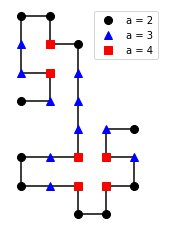
\includegraphics[width=3cm, keepaspectratio=True]{Images/count.png}
\caption{A conformation with $N=26$ monomers. Here $n_2=10$, $n_3=$\textbf{XXX}
and $n_3=$\textbf{YYY}. Monomers are marked according to the numnber of nearest neighbors: 
black circles are two neighbors, blue triangles are three neighbors and red squares
are four neighbors.}
\label{fig:2-3-4}
\end{figure}


Denoting by $n_\alpha$ the fraction of monomers with $\alpha$ neighbors, 
for a length-$N$ conformation on a lattice with the coordination number $z$
we find
%
$$
\sum_{\alpha=2}^z n_\alpha = 1 - n_1 \;,
\label{eq:sum_n}
$$
%
where the second term accounts for the two end monomers: $n_1 \leqslant 2/N$.


%%%%%%%%%%%%%%%%%%%%%%%%%%%%%%%%%%%%%%%%%%%%%%%%%%%%%%%%%%%%%%%%%%%%%%%%%%%%%%%%
\subsubsection{2D square lattice, $z=4$}

Since Eq.\ \eqref{eq:sum_n} holds for any conformation of $N$ monomers, we
compute the average values of $n_\alpha$ under the Gibbs distribution \eqref{eq:Z}.
We start with the limit of $J=0$, which is nothing but a usual non-interacting SAW model.
(The Gibbs distribution \eqref{eq:H_Ising_ISAW}-\eqref{eq:Z}
becomes uniform for $J=0$).

Fig.\ \ref{fig:finite_size_SAW} shows the mean values of $n_\alpha$ with $\alpha=2, 3, 4$
for a SAWs of varying lengths on a 2D square lattice (with $z=4$).
For short lengths, $N \leqslant 11$, we enumerate all SAW conformations and
average the values of $n_\alpha$; for larger values of $N$ we use Monte Carlo simulations.
%
\begin{figure}[h!]
    \centering
    \includegraphics[width=0.99\textwidth]{Images/ISAWJ0_Bulk2-4.png}
    \caption{Fractions of monomers, $n_\alpha$, of the SAW
model (Eqs.\ \eqref{eq:H_Ising_ISAW}-\eqref{eq:Z} with $J=0$) on a square lattice as a function
of $1/N$. Black dots are results of exact enumeration for $N = 5$ to $N=11$; 
open squares are results MC simulations. See text for discussion.}
    \label{fig:finite_size_SAW}
\end{figure}
%

Fig. \ref{fig:finite_size_SAW} shows that $n_\alpha$ ($\alpha=2, 3, 4$) saturate
at large $N$ with some finite-size corrections. The most noteworthy feature of
Fig.\ \ref{fig:finite_size_SAW} is that the ``surface'' fraction
%
$$
n_3 \to 0.25 \qquad\text{as\quad}N\to\infty \;,
$$
%
so that asymptotically $N/4$ monomers of a length-$N$ SAW conformation are ``surface-like'' and
$3 N/4$ monomers are ``1D-like''.


Fig.\ \ref{fig:Ising_vs_ISAW2D} shows results of MC simulations for
$n_\alpha$ as functions of the coupling constant $J$ across the collapse transition
for both ISAW model and Ising-ISAW model \eqref{H_Ising_ISAW}.
We see that for the lengths $N > 1000$, finite-size corrections are barely visible.
For the ISAW model,  the fraction of the ``2D-like'' monomers, $n_4$, is
essentially zero for small $J$ and quickly increases on approach to the $\theta$-point.
For the Ising-ISAW model, the behavior is qualitatively similar, if somewhat
more smooth for $J < J_\theta$. The ``1D-like'' fraction, $n_2$ is also a smooth
monotonic function across the whole range of $J$. 

On the contrary, the ``surface-like'' fraction, $n_3$,---for both models---develops
a peak in the vicinity of the respective collapse transitions. The available MC
data suggest that the peak becomes more narrow as $N$ increases, and that the
position of the peak is shifted away from the $\theta$-point.


\begin{figure*}
    \centering
    \includegraphics[width=0.99\textwidth]{Images/bulk2-4_inset.png}
    \caption{Fractions of monomers of Ising-ISAW model (squares) and ISAW model (stars) on a square lattice with 2-4 nearest neighbors as function of $J$ with length of conformations $N = $ 1000 (blue), 2500 (yellow), 3600 (green), 4900 (red). Black vertical line define point of $\theta$-transition for ISAW model \cite{Caracciolo2011}, red line - for Ising-ISAW model \cite{faizullina2021critical, Foster2021}. Reproduced from Ref.\cite{faizullina2021critical}}
    \label{fig:Ising_vs_ISAW2D}
\end{figure*}



%%%%%%%%%%%%%%%%%%%%%%%%%%%%%%%%%%%%%%%%%%%%%%%%%%%%%%%%%%%%%%%%%%%%%%%%%%%%%%%%
\subsubsection{3D cubic lattice($z=6$) }

On a 3D cubic lattice with the coordination number $z=6$, the classification of a
local neighborhoods is more complicated than that on a 2D square lattice.
``1D-like'' monomers still have two neighbors, deep bulk corresponds to six
neighbors. Considering a cube-shaped globule, three neighbors define ``corners'',
and faces of a cube have five neighbors.
Since typical conformations are not perfect cubes, it is reasonable to expect
that $n_6$ corresponds to the ``bulk-like'' monomers and
$n_3$, $n_4$ and (to some extent) $n_5$ correspond to ``surface-like'' monomers.

Fig. \ref{fig:Ising_vs_ISAW} shows our MC results for the 3D cubic lattice in the
left column. Here we simulate conformations of up to $N=600$ for both models,
Ising-ISAW \ref{H_Ising_ISAW} and ISAW \ref{XXX}.

For the Ising-ISAW model, Fig.\ \ref{fig:Ising_vs_ISAW} shows that the
``1D-like'' and ``bulk-like'' fractions, $n_1$ and $n_6$, respectively,
are monotonic and develop a jump at the critical coupling at increasing $N$, which is
consistent with the first-order character of the transition \cite{Garel1999, Foster2021}.

The ``surface-like'' fractions $n_3$ and $n_4$ clearly develop a peak in the
critical region, which becomes progressively more narrow and better defined 
at increasing $N$, Finite-size corrections are strong for the available values of $N$. 

Our MC data for $n_5$ can be interpeted as
finite-$N$ corrections to either a jump or a peak. Simulations for 
larger lengths $N$ are needed to conclusively resolve the behavior of $n_5$
in the critical region. 

For the ISAW model the begavior is qualitatively similar: the ``bulk-like''
fraction, $n_6$, is essentially zero all the way up to the theta-transition $J_\theta =...$\textbf{XXX}
and is monotonically increasing for $J > J_\theta$, the ``1D-like'' fraction $n_2$
decreases monotonically with $J$---for the available lengths $N$, the behavior
is almost featureless. The ``surface-like'' fractions $n_3$ and $n_4$ develop
a peak which shifts towards $J_\theta$ as $N$ increases, and $n_5$ is very
slowly developing what is probably a peak. 
The overall dependence if $n_\alpha$ on $J$ for the available lengths
$N \leqslant 600$ is much slower for the ISAW model than for the Ising-ISAW
model, which is consistent with a continuous collapse transition with tricritical
exponents \cite{Vanderzande}.

Comparing the behavior of the ISAW and Ising-ISAW models on the 3D cubic lattice,
we conclude that the dependence of the ``surface-like'' fraction is sensitive
to the nature of the collapse transition: for the ISAW model, where the transition
is continuous, the finite-size corrections are much stronger than those for the
Ising-ISAW model, where the transition is first-order. \textbf{XXX: into the sconclusion}

\textbf{TODO: 0.25, hypercubic}

%%%%%%%%%%%%%%%%%%%%%%%%%%%%%%%%%%%%%%%%%%%%%%%%%%%%%%%%%%%%%%%%%%%%%%%%%%%%%%%%
\subsubsection{2D triangular lattice($z=6$) }

In this section, we consider the ISAW and Ising-ISAW models on the 2D triangular
lattice, which has a coordination number $z=6$. Despite having the same coordination
number as a 3D cubic lattice, the triangular lattice structure is rather
different for the SAW-like conformations because a one-dimensional line forms
and impenetrable boundary on a triangular lattice but not on a cubic lattice. 
Monomers with one and six neighbors still can be interpreted as ``1D-like'' and
``bulk-like'', respectively, but the straight boundary corresponds to four neighbors.
This way, the interpretation of the fraction $n_3$ is not entirely clear-cut: it is
neither ``1D-like'', nor does it correspond to a right boundary.
We can thus expect that the ``surface-like'' behavior is displayed by the fractions
$n_4$ and $n_5$.

Fig.\ \ref{fig:Ising_vs_ISAW} shows results of MC simulations in the right-hand
column. For the ISAW model (open symbols) the fractions $n_2$ and $n_3$ are
monotonically decreasing functions of $J$. The ``surface-like'' fractions, $n_4$ and $n_5$
develop broad peaks which get progressively sharper with increasing $N$. The peak
locations are not far from the extimate of the collapse transition
$J_{t} = 0.405 \pm 0.07 of Ref.\ $\cite{Privman1986}. The bulk fraction $n_6$
is a featureless monotonically increasing function of $J$ for the available lengths
$N \leqslant 600$. 

For the Ising-ISAW model the behavior is qualitatively similar, with the location
of the peaks of $n_4$ and $n_5$ suggesting that the collapse transition occurs
around $J_t \approx 0.6$. We are not aware of an independent estimate of the
location of the collapse transition for the Ising-ISAW model on a trinagular lattice.

Comparing the Ising-ISAW and ISAW models, we see that in the latter model,
the finite-size dependence is smoother than in the former, suggesting that the
crossover exponent, which governs the size of the critical region, 
is larger for the ISAW model.


Finally, we consider the $J=0$ limit.
\textbf{1. No 1/4 --- specific for hypercubic lattices?
2. Note that n=2 and n=3 are both equal 0.36, are they?
}

------------------------





In this section we studied proportions of monomers with fixed numbers of nearest neighbors for Ising-ISAW and ISAW models on 3D-square and 2D-triangular lattices. Monomers of all four modified models can have from 2 to 6 close-range energy connections and some types of monomers, according to number of connections they have, can be interpreted similarly: for example, it is obvious that parts of conformations with monomers with only two nearest neighbors represent 1D-conformations or chains whatever lattice was used in observed model. And the opposite - regions where monomers have maximum number of close-range connections represent densely packed areas deep inside the globule. Talking about cubic lattice, other types of monomers can be also interpreted: monomers with only three neighbors define "corners" on conformation, while only monomers on a cube edge (or it also can be on a isolated plane from other part of globule) can have four neighbors. Presence on five neighbors belongs to the monomers on a surface of conformation. Unfortunately, we cannot make similar interpretations for conformations on a triangular lattices.

To begin with, we performed simulations of ISAW model on square lattice on lengths from 5 to 3600 at $J=0$ with collecting statistics for fraction of monomers with 2 to 4 neighbors. To understand we mechanics of calculating neighbors of monomers, we also manually enumerated fractions of monomers with these number of neighbors for short conformations (5 to 11). Our results matched.


\subsubsection{Ising model on a SAW-conformation}

Using method of MC simulations from Ref. \cite{faizullina2021critical}, we enumerated proportions of monomer with 2-6 nearest neighbors in Ising-ISAW model on a three-dimensional square (or cubic) lattice.

As it is seen from left part of \Cref{fig:Ising_vs_ISAW}, increasing the strength of nearest-neighbors interaction J leads to conformation becoming more dense as proportions of monomers with higher numbers of close-range connections significantly increases after $\theta$-transition located in a blue zone (for Ising-ISAW model on a cubic lattice $T_{c} = 0.5263 \pm 0.055$\cite{Foster2021}) (see \Cref{tab:Ising_T_c}).

We also repeated MC simulations for two-dimensional triangular lattice. Unlike the 3D-square lattice, the 5-th and 6-th possible neighbors located on the same plane as the first four, so conformations are expected to be more dense on this lattice.

% здесь был TrIsing_complex

\textbf{TODO: include}
Critical region of the model on a triangular lattice was not enumerated yet. But as it was suggested, density of conformations becomes higher as nearest-neighbors interaction $J$ strengthen. Moreover, proportion of monomers with six neighbors on a triangular lattice is far higher than on a cubic one. It is also significant that "triangular" conformations with no inner interaction have almost twice shorter one-dimensional chains than conformations on a cubic lattice in the same conditions.

\subsubsection{ISAW model}

To understand how the presence of magnetic properties affects on density of models, we also performed Monte-Carlo simulations on a parental model of self-avoiding walks on the same lattices. Results was similar to Ising-ISAW model, as suggested from "parent" model. For cubic lattice $T_{c} = 0.2779\pm 0.0041 $\cite{Tesi1996}. For the trianglular lattice, $J_{c} = 0.405 \pm 0.07 $\cite{Privman1986}. \Cref{fig:Ising_vs_ISAW} shows that geometric aspects of phase transition in ISAW model manifect earlier than in Ising-ISAW ones.  

\begin{figure}
    \centering
    \includegraphics[width=0.95\textwidth, height=22.5cm]{Images/Ising_vs_ISAW.png}
    \caption{Fractions of monomers of Ising-ISAW model (stars) and ISAW model (open squares) on a cubic lattice (left column) and 2D-triangular lattice (right column) with 2-6 nearest neighbors as function of $J$ with length of conformations $N = $ 100 (green), 300 (blue) and 600 (red). Vertical lines define points of $\theta$-transition (For cubic lattice: black line for ISAW model \cite{Tesi1996} and blue line for Ising-ISAW model \cite{Foster2021}; for triangular lattice: blue line for ISAW model \cite{Privman1986})}
    \label{fig:Ising_vs_ISAW}
\end{figure}

% здесь были графики по ISAW

\section{Discussion}

\section{Acknowledgments}

\newpage

\bibliography{bibliography}

\end{document}
